\chapter{Reinforcement Learning} % {Theoretical foundations}
\label{chap:RL}


\section{Introduction}


As described in \cite{SuttonBarto}, Reinforcement Learning (\acrshort{rl}) is a paradigm of Machine Learning (\acrshort{ml}), along with others, like supervised learning and unsupervised learning. It analyzes how it is possible to learn the best course of action in an environment based on maximizing some given numerical reward. The learner is not told which actions to take, but learns empirically which are the ones that lead to a bigger reward. It is also possible that the current action influences not only the immediate reward, but also the next status of the environment, and, through that, all the other rewards to come. In this case, we speak of delayed reward, which, together with trial-and-error search, form the two distinctive features of \acrshort{rl}.

\begin{figure}[!ht]
    \centering
    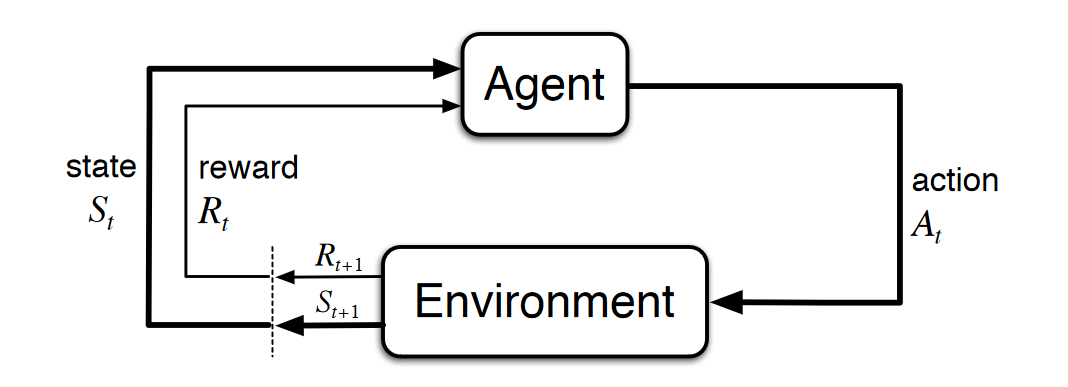
\includegraphics[width=0.9\textwidth]{chapters/figures/MDP-diagram.png}
    \caption{The agent-environment interaction \cite{SuttonBarto}}
    \label{fig:MDP}
\end{figure}

In an \acrshort{rl} problem we have a learning \emph{agent}\index{agent}, the decision-maker, that interacts over time with the \emph{environment}\index{environment} in which it is placed --- which includes everything outside the agent --- in order to achieve a \emph{goal}\index{goal}, which is to maximize the total reward it receives over the long run. As we see in \autoref{fig:MDP}, the agent can sense aspects of its environment through the \emph{states}\index{state} --- which can also be seen as a representation of the environment itself, it can choose \emph{actions}\index{action} to influence the environment, and it receives a \emph{reward}\index{reward} based on the outcome of its actions. We consider to be a reinforcement learning method any method that is well suited to solving problems framed in this way. Other elements of the \acrshort{rl} system are a \emph{policy}, a \emph{value function}, and a \emph{model} of the environment. A \emph{policy}\index{policy} describes the behavior of the agent at a given time, using a mapping from states to actions to be taken in those states. A \emph{value function}\index{value function} determines the value of a state as the total amount of reward an agent can expect to accumulate over the future, starting from that state. Instead, a \emph{model} of the environment\index{model of the environment} reproduces the behavior of the latter, and it is used for planning actions before actually experiencing them. For example, given to the model a state and action, it might predict with a certain probability the resultant next state and next reward.


\section{Finite Markov Decision Processes}

The treatment of this topic will closely follow the one presented in \cite{SuttonBarto}.

\emph{Markov Decision Processes}\index{Markov Decision Process}, or \acrshort{mdp}s, are used to formalize sequential decision-making, where actions influence the given rewards and the next states of the system, and through the latter also future rewards can be affected. Thus, \acrshort{mdp}s need to balance both immediate and delayed rewards. This formalism is used both in decision-theoretic planning (\acrshort{dtp}), \acrshort{rl}, and other learning problems in stochastic domains \cite{WierOtter12RLStateOfTheArt}.

We assume that the process evolves through a sequence of discrete time steps, $t = 1, 2, 3, \ldots$, even if it is possible to extend to the continuous case. These steps do not need to reflect fixed intervals of real time, but they can refer to arbitrary successive stages of decision-making and acting. At each time step $t$, the agent detects the \emph{state} of the environment, $S_t \in \mathcal S$, based on which it selects an action $A_t \in \mathcal A(s)$ (if the action set is the same in all states, we will write it simply as $\mathcal A$). Then, as a consequence, the agent receives, one time step later, a numerical reward $R_{t+1} \in \mathcal R \subset \mathbb R$, and ends up in a new state $S_{t+1}$. Thus, given this sequential process, it emerges a sequence, or \emph{trajectory}\index{trajectory}, given from
\begin{equation}
    S_0, A_0, R_1, S_1, A_1, R_2, S_2, A_2, R_3, S_3, \ldots
\end{equation}

In a \emph{finite} \acrshort{mdp}\index{finite MDP} we have that the set of states $\mathcal S$, actions $\mathcal A$, and rewards $\mathcal R$ have finite cardinalities, respectively $|\mathcal S|, |\mathcal A|$, and $|\mathcal R|$.

Since it is a \textit{finite} MDP, the random variables $R_t$ and $S_t$ have well-defined discrete probability distributions, and since we are considering a \textit{Markov} process, it holds the \emph{Markov property}, also called \emph{memorylessness property}, and thus the \emph{dynamics}\index{dynamics} of the process through the space of states, or the \emph{model} of the environment\index{model of the environment}, depend only on the preceding state and action:
\begin{equation}
    p(s', r \mid s, a) := \text{Pr}\{S_t = s', R_t = r \mid S_{t-1} = s, A_{t-1} = a\} \, ,
    \label{eq:transitions}
\end{equation}
for all $s', s \in \mathcal S$, $r \in \mathcal R$, and $a \in \mathcal A(s)$.

One could compute also the \emph{transition probabilities}\index{transition probabilities}, defined (with a little abuse of notation, since we continue to use the letter $p$) as
\begin{equation}
    p(s'|s, a) := \text{Pr}\{S_t = s' \mid S_{t-1} = s, A_{t-1} = a\} = \sum_{r \in \mathcal R} p(s', r \mid s, a) \, .
\end{equation}

The \emph{expected rewards}\index{expected reward} for state--action--next-action triples can be computed as $r: \mathcal S \times \mathcal A \times \mathcal S \to R$,
\begin{equation}
    r(s, a, s') := \mathbb E \left[ R_t | S_{t-1} = s, A_{t-1} = a, S_t = s' \right] = \sum_{r \in \mathcal R} r \cdot p(s', r | s, a) \, .
\end{equation}

The \acrshort{mdp} can also be seen as the tuple $(\mathcal S, \mathcal A, p, r)$, where $r = r(s,a,s')$ is the expected immediate reward that the agent receives for taking action $a$ in state $s$ \cite{Kaelbling1998, Uther2010}.

To describe how likely it is for an agent to take any given action from any given state, we use the notion of policy. A \emph{policy}\index{policy} is a class of probability distributions $\pi(a|s)$ over an action $a \in A(s)$ for each state $s \in \mathcal S$:
\begin{equation}
    \pi(a|s) = \text{Pr} \{A_t = a | S_t = s\} \, ,
    \label{eq:policy-theory}
\end{equation}
which describes the probability that the agent chooses that action being in that state at that time step $t$.

The agent's goal is to maximize the \emph{expected return}\index{expected return}, o \emph{cumulative reward}\index{cumulative reward|see {expected return}}, it receives in the long run given a certain policy $\pi$:
\begin{equation}
    \mathbb E [G_t] = \mathbb E_{p(\cdot,\cdot|s_t,a_t), \pi} \left[ \sum_{t=0}^\infty \gamma^t R_t \right].
    \label{eq:goal}
\end{equation}
where $\gamma \in [0,1]$ is the \emph{discount factor}\index{discount factor}, and it determines how much we value future rewards. With $\gamma = 0$ the agent considers only immediate rewards and discards future ones, while with $\gamma = 1$ the agent will take into account, in the same way, every reward it receives, considering a very long series of events.

Actually, we can take this average with respect to the distribution of rewards themselves, so as to ignore the dependency on the distribution of rewards. This is a distinctive property of the fact that we are working with a \textit{known model of the environment}. So, since we are only interested in optimizing averages, we do not care any longer about what is the actual distribution of the rewards. Thus, we can rephrase the agent goal as
\begin{equation}
    \mathbb E [G_t] = \mathbb E_{p(\cdot|s_t,a_t), \pi} \left[ \sum_{t=0}^\infty \gamma^t r(s, a, s') \right].
    \label{eq:goal-average}
\end{equation}

To reach its goal, the agent must estimate how good it is to be in a given state if it is following a certain policy. This value is stored in the \emph{(state-)value function}\index{value function}\index{state-value function|see {value function}}. Formally, the value of state $s$ under policy $\pi$ is
\begin{equation}
    V_\pi (s) := \mathbb E \left[ G_t \mid S_t = s \right] = \mathbb E \left[ \left. \sum_{t=0}^\infty \gamma^k R_t \, \right| \, S_t = s \right], \; \text{for all } s \in \mathcal S \, ,
\end{equation}
which is the expected return when starting in state $s$ and following policy $\pi$ thereafter. If there exists a terminal state\index{terminal state}, which causes the process to terminate if reached, its value is always zero.

Similarly, the value of taking action $a$ in state $s$ under policy $\pi$ is stored in the \emph{(state-)action value function}\index{action value function}\index{state-action value function|see {action value function}}, or \emph{quality}\index{quality|see {action value function}}, which is expressed with
\begin{equation}
    \begin{aligned}
        Q_\pi(s,a)
        &:= \mathbb E \left[ G_t \mid S_t = s, A_t = a \right] \\
        &= \mathbb E \left[ \left. \sum_{t=0}^\infty \gamma^k R_t \, \right| \, S_t = s, A_t = a \right],
    \end{aligned}
    \label{eq:Q}
\end{equation}
which is the expected return starting from state $s$, taking action $a$ and following policy $\pi$ thereafter.

We have that the following relation holds:
\begin{equation}
    V_\pi(s) = \sum_a \pi(a|s) Q_\pi(s,a) \, .
\end{equation}

The value function possesses a fundamental property, which is extensively used in \acrshort{rl}: it satisfies the following recursive relation
\begin{equation}
    \begin{aligned}
        V_\pi (s)
        &= \sum_a \pi(a|s) \sum_{s', r} p(s', r \mid s, a) \left[ r + \gamma V_\pi (s') \right] \\
        &= \sum_a \pi(a|s) \sum_{s'} p(s' \mid s, a) \left[ r(s,a,s') + \gamma V_\pi (s') \right] \, ,
    \end{aligned}
\end{equation}
which is called \emph{Bellman equation for $V_\pi$}\index{Bellman equation}.

Similarly, we have the \emph{Bellman equation for $Q_\pi$}:
\begin{equation}
    \begin{aligned}
        Q_\pi (s, a)
        &= \sum_{s', r} p(s', r \mid s, a) \left[ r + \gamma \sum_{a'} \pi(a'|s')  Q_\pi (s', a') \right] \\
        &= \sum_{s'} p(s' \mid s, a) \left[ r(s,a,s') + \gamma \sum_{a'} \pi(a'|s')  Q_\pi (s', a') \right] \, .
    \end{aligned}
    \label{eq:Q-recursive}
\end{equation}


\section{Partially Observable MDPs}

The presentation of this topic will mainly follow the one in \cite{Spaan12pomdp}.

What happens if the agent does not know anymore with full certainty the state of the environment, maybe due to imperfections or limitations in the agent's sensors, or to errors in the interpretation of the environment, or simply to unknown aspects of the environment itself?

If some features of the state are hidden from the agent, and the latter can sense only a part of the real state of the environment, the resultant state signal will no longer be Markovian, breaking a key assumption of most \acrshort{rl} methods, like the \acrshort{mdp} formulation. Luckily, we can consider an extension of the (fully observable) \acrshort{mdp} framework, that can deal with the uncertainty originating from the imperfect states perceived by the agent or the uncertain action effects.

A \emph{partially observable Markov decision process}\index{partially observable Markov decision process}, or \acrshort{pomdp}, is a framework that considers environments that are only partially observable to the agent, but allows anyway for optimal decision-making \cite{Kaelbling1998}, contrary to the requirement of full knowledge of the environment of \acrshort{mdp}s.

The fact that the environment is partially observable can derive mainly from two reasons:
\begin{itemize}
    \item different states generate the same observation, due to the same sensor reading, caused by the agent's limited knowledge of the environment;
    \item sensor readings are noisy, so the same state can generate different observations due to different sensor readings.
\end{itemize}
Thus, we have that the state of the environment is not uniquely identified by the agent's observations, and situations that appear similar to the agent may require instead different actions.

Interestingly, we can consider fully observable \acrshort{mdp}s as a special case of \acrshort{pomdp}s, in which the observation function maps each state to its correct unique observation deterministically \cite{Poupart2010}.

\begin{figure}[ht]
    \centering
    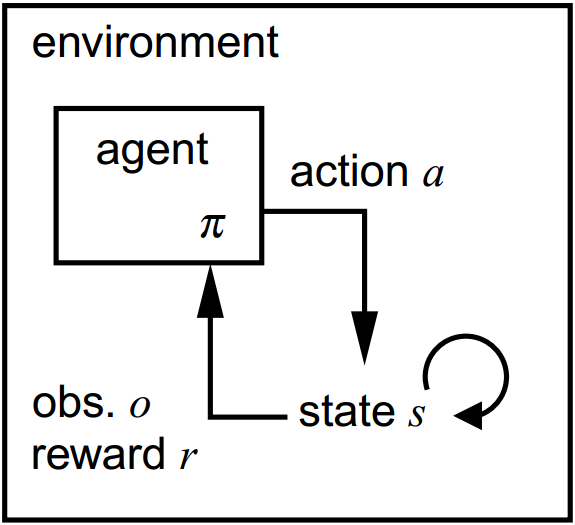
\includegraphics[width=0.45\textwidth]{chapters/figures/POMDP-schema.png}
    \caption{The agent-environment interaction in a POMDP \cite{Spaan12pomdp}}
    \label{fig:POMDP}
\end{figure}

Since a \acrshort{pomdp} is an extension of an \acrshort{mdp}, they share many elements. Also in \acrshort{pomdp}s the time is divided into different steps, and in each one of them the agent has to take an action. As for the \acrshort{mdp}s, we will consider discrete and finite models, which are simpler than the continuous ones. So the environment is represented with a finite set of states $\mathcal S = \{ s_0, s_1, s_2, \ldots, s_N \}$, and the finite set of possible actions is $\mathcal A = \{a_0, a_1, \ldots, a_K\}$. But instead of perceiving directly the state in which the environment is, the agent senses an \emph{observation}\index{observation} of it --- a signal that depends on the true state of the system but provides only partial information about it. The set of observations is discrete and finite: $\mathcal O = \{o_0, o_1, \ldots, o_M\}$, and represents all the possible sensor readings the agent can receive.

If the system is in state $s$ and the agent performs action $a$, we have that the system transitions to state $s'$ according to the transition probability $p(s' | s, a)$ as in a \acrshort{mdp}, but the agent receives observation $o'$ with probability
\begin{equation}
    z(a,s',o') = \text{Pr}(o' | a, s') \, ,
\end{equation}
using the notation of \cite{Poupart2010}.

\autoref{fig:POMDP} represents the interaction between these elements in the \acrshort{pomdp}.

Thus, a \acrshort{pomdp} can be described as the tuple $(\mathcal S, \mathcal A, p, r, \mathcal O, z)$, where $r = r(s,a,s')$ is the expected immediate reward, as in an \acrshort{mdp} \cite{Kaelbling1998}.

The goal of the agent is, once again, to find the optimal policy $\pi$ that maximizes the expected return\index{expected return} in \eqref{eq:goal-average}. To solve both \acrshort{mdp}a and \acrshort{pomdp}s, one can use several different methods, which are classified according to the dimensions of the state and action spaces, as well as based on whether the model of the environment is available or not. In fact, there are \emph{tabular methods}\index{tabular methods} --- which are exact and use arrays to store value functions, or \emph{approximate solution methods}\index{approximate solution methods} --- which employ function approximators, using limited computational resources; then there are \emph{model-based methods}\index{model-based methods} --- which make use of the known model of the environment and of planning to find the exact optimal policy, or \emph{model-free methods}\index{model-free methods} --- which are trial-and-error learner.

Often finding an exact optimal policy for \acrshort{pomdp}s can be computationally very expensive, so even for relatively small problems it is required to use approximate methods \cite{Aberdeen2002ScalingIP}. They are divided into two main classes: \emph{value-function methods}\index{value-function methods} --- or \emph{action-value methods}\index{action-value methods|see {value-function methods}} as in \cite{SuttonBarto}, that attempt to learn an approximate value function of the belief\index{belief} states (which are probability distributions over the states); and \emph{policy-based methods}\index{policy-based methods}, that search for a good policy within a fixed class of parameterized policies. We will focus on the second ones, since it is what we will implement to solve our problem.


\section{Policy gradient methods}
\label{sec:pgm}

A \emph{policy gradient method}\index{policy gradient method} is a policy-based method that attempts to optimize the parameters of a parametrized policy using either \emph{gradient  ascent}\index{gradient ascent} or \emph{gradient descent}\index{gradient descent} in the parameters' space, based on the expression of the agent's goal. In fact, it tries to maximize (or minimize) the expected return of a policy inside the policy class dictated by the parametrization. This method then uses directly the policy to choose the actions, instead of consulting a value function, which however might still be used to learn the parameters.

Policy gradient methods present some perks that make them highly valuable: the parametrized policy allows for direct incorporation of potential environment insights, they can naturally switch from the discrete setting to the continuous one, and they converge to at least a locally optimal policy, even if, as a drawback, the convergence can be very slow and finding the global optimum instead of a local one can be hard \cite{Peters2010}. Another distinctive trait of these methods is that they can also naturally handle partial state information. In fact, if a state variable can not be observed, then we can choose the policy parametrization such that the parameters do not depend on that state variable. Thus, we can directly apply these methods to \acrshort{pomdp}s, without having to make any changes.

We will denote the policy's parameters' vector with $\boldsymbol \theta \in \mathbb R^{d'}$, and we will write, as in \eqref{eq:policy-theory},
\begin{equation}
    \pi(a|s,\boldsymbol \theta) = \text{Pr}\{A_t = a | S_t = s, \boldsymbol \theta_t = \boldsymbol {\theta}\} \, ,
    \label{eq:policy-with-parameters}
\end{equation}
for the probability of taking action $a$ being in state $s$ at time $t$ with parameters $\boldsymbol \theta$ \cite{SuttonBarto}. The policy can be parametrized in any way, as long as it is differentiable with respect to its parameters, which means that the column vector of partial derivatives of $\pi$ w.r.t. the components of the parameters' vector $\boldsymbol \theta$, $\nabla_{\boldsymbol \theta} \pi (a|s,\boldsymbol \theta)$, exists and is finite for all $s \in \mathcal S, a \in \mathcal A$ and $\boldsymbol \theta \in \mathbb R^{d'}$. In particular, as described in \cite{Peters2010}, for discrete problems is often used the (exponential) soft-max distribution (i.e., Gibbs or Boltzmann distribution)
\begin{equation}
    \pi(a|s, \boldsymbol \theta) = \frac{e^{\phi(s,a)^\top \boldsymbol \theta}}{\sum_{b \in \mathcal A} e^{\phi(s,b)^\top \boldsymbol \theta}} \, ,
    \label{eq:pi-boltzmann}
\end{equation}
while for continuous problems it is used the Gaussian distribution
\begin{equation}
    \pi(a|s, \boldsymbol \theta) = \mathcal N(\phi(s,a)^\top \boldsymbol \theta_1, \boldsymbol \theta_2) \, ,
\end{equation}
where $\boldsymbol \theta_2$ is an exploration parameter, and $\phi(s,a) \in \mathbb R^{d'}$ is a feature vector characterizing state $s$ and action $a$ \cite{Sutton2000}.

To learn the policy parameters $\boldsymbol \theta$ we will use the  gradient of some scalar \emph{performance measure}\index{performance measure} $J_\pi(\boldsymbol \theta)$ --- which can also be directly the expected return --- with respect to the policy parameters. If the performance $J_\pi(\boldsymbol \theta)$ measures the rewards that the agent receives, we want to maximize it, so we update the parameters approximating gradient \textit{ascent} in $J_\pi(\boldsymbol \theta)$:
\begin{equation}
    \boldsymbol \theta_{k+1} = \boldsymbol \theta_k + \alpha \nabla_{\boldsymbol \theta} J_\pi(\boldsymbol \theta_k) \, ;
    \label{eq:grad-ascent}
\end{equation}
instead, if the performance measures the costs that the agent encounters, we seek to minimize it, so we use approximate gradient \textit{descent} in $J(\boldsymbol \theta)$:
\begin{equation}
    \boldsymbol \theta_{k+1} = \boldsymbol \theta_k - \alpha \nabla_{\boldsymbol \theta} J_\pi(\boldsymbol \theta_k) \, ;
    \label{eq:grad-descent}
\end{equation}
where, in both cases, $\alpha > 0$ is a \emph{step-size parameter}\index{step-size parameter|see {learning rate}} or the \emph{learning rate}\index{learning rate}.

As done before, we will treat the episodic case, for which we define the \emph{performance measure}\index{performance measure} $J_\pi(\boldsymbol \theta)$ as the average value of the initial states\index{initial state} of the process:
\begin{equation}
    \begin{aligned}
        J_\pi (\boldsymbol \theta) 
        &= \sum_s \rho_0(s) V_{\pi_{\boldsymbol \theta}}(s) \\
        &= \sum_s \rho_0(s) \sum_a \pi(a|s) Q_{\pi_{\boldsymbol \theta}}(s, a) \, .
    \end{aligned}
    \label{eq:J}
\end{equation}
where we define as $\rho_0(s')$ the probability that an episode begins in state $s' \in \mathcal S$.

Let us define $\eta_\pi(s')$ as the average number of time steps that the agent spends in state $s'$ before the process dies. Time is spent in a state $s'$ if episodes start in that state $s'$, or if the environment transitions into $s'$ from a previous state $s$ in which time is spent. Thus, we have that the formula for $\eta_\pi$ is
\begin{equation}
    \eta_\pi(s') = \rho_0(s') + \sum_s \eta_\pi(s) \sum_a \pi(a|s) p(s'|s, a), \; \text{for all } s' \in \mathcal S.
    \label{eq:eta}
\end{equation}
This is a \textit{linear system} of equations, one for each state $s' \in \mathcal S$, and it can be solved for the expected number of visits $\eta_\pi(s)$.

The \emph{policy gradient theorem}\index{policy gradient theorem} provides an analytic expression for the gradient of the performance $J$ with respect to the policy parameters, which is what we need to approximate for gradient ascent in \eqref{eq:grad-ascent} (or descent in \eqref{eq:grad-descent}):
\begin{equation}
    \nabla_{\boldsymbol \theta} J(\boldsymbol \theta) = \sum_s \eta_\pi(s) \sum_a Q_\pi(s, a) \nabla_{\boldsymbol \theta} \pi(a|s).
    \label{eq:gradJ}
\end{equation}
See \cite{SuttonBarto} for the demonstration in the episodic case, which involves just elementary calculus and re-arranging of terms in the expression of the value function $V_\pi$.

Thus, solving the expression for \eqref{eq:gradJ} and using it in equations \eqref{eq:grad-ascent} -- \eqref{eq:grad-descent} allows optimizing the parameters of the policy, building an optimal policy in the chosen parametrization class. Note that to find both $\eta_\pi$ and $Q_\pi$ we need to solve two linear systems, \eqref{eq:Q-recursive} and \eqref{eq:eta}, and, moreover, they depend on the policy $\pi$, thus they must be solved at every iteration.


%\subsection{Natural policy gradient}

% See Natural actor critic, Peters, Vijayakumar, Schaal, European Conference on Machine Learning (2005).

% See (Hennes, Neural Replicator Dynamics: Multiagent Learning via Hedging Policy Gradients) \href{https://arxiv.org/pdf/1906.00190.pdf}{here} (page 8, appendix A4) for proof of natural gradient.

% Amari, S. I. (1998). Natural gradient works efficiently in learning. Neural Computation, 10(2):251–276.